%----------------------------------------------------------------------------------------
% HOE GOED IS HET MODEL? Alle opgaven zijn eigen werk; alle gegevens zijn verzonnen, behalve het kwartet
% van Anscombe (1973).
%
% Opbouw: Probleem, Start, leerstof (theorie, werkwijze of uitleg, voorbeeld, korte oefening), en op een
% nieuwe pagina de Opdrachten (door elkaar, stijgende moeilijkheid), Koppel en Test jezelf.
% Labels van dit hoofdstuk beginnen met h2-.
%----------------------------------------------------------------------------------------

\mychapter{2}{Hoe goed is het model?}

\begin{probleem}
\naast{Op een hete zomerdag meet een student om 15 uur de temperatuur in tien straten van haar stad. Ze schat ook welk deel van elke straat onder het bladerdek van bomen ligt (in procent).

\smallskip
\kleinetabel[$x$ (\%)][$y$ (°C)]{10}{5 & 12 & 18 & 25 & 30 & 38 & 45 & 52 & 60 & 70}{35{,}3 & 34{,}5 & 34{,}9 & 33{,}5 & 34{,}0 & 33{,}9 & 32{,}9 & 32{,}4 & 33{,}1 & 31{,}8}

\smallskip
Straten met meer bomen zijn koeler, maar de punten liggen niet op een rechte. Hoeveel van de verschillen in temperatuur verklaart het bladerdek? Kan het verband toeval zijn, met maar tien straten? En hoeveel graden koeler is een straat met 10 procentpunt meer bladerdek, met een betrouwbaarheidsinterval?}{\begin{tikzpicture}[x=.062cm,y=.68cm,font=\scriptsize]
  \diagram[$x$ (\%)][$y$ (°C)]{0}{10}{70}{31}{1}{36}
  \xas{0,20,...,60}\yas{31,32,...,36}
  \punten[inkt]{(5,35.3) (12,34.5) (18,34.9) (25,33.5) (30,34.0) (38,33.9) (45,32.9) (52,32.4) (60,33.1) (70,31.8)}
\end{tikzpicture}}
\end{probleem}

\lkr{Leerplan Complementair (III-WiCo-d): LPD 52, de wenk over de determinatiecoëfficiënt $R^2$ als verhouding van de verklaarde tot de totale variantie, met een tekening, en LPD 51 (het enkelvoudig lineair regressiemodel toepassen om de invloed van een variabele op een andere te onderzoeken). Het bewijs dat $R^2 = r^2$ legt al de link met LPD 54 (multivariate statistiek). De residuplot, het kwartet van Anscombe, de t-toets en het betrouwbaarheidsinterval voor de helling zijn de invulling van \textit{de invloed onderzoeken}; de toets steunt op de t-verdeling uit Kansverdelingen, hoofdstuk 3 (LPD 49). Wie die module niet zag, kent uit Statistiek de p-waarde en het betrouwbaarheidsinterval met de normale verdeling: geef dan kort uit Kansverdelingen dat $t^*$ en \texttt{tcdf} een verdeling met dikkere staarten gebruiken. Op de TI-84: \texttt{LinRegTTest} in STAT, TESTS; let op dat het toestel daar $y = a + bx$ schrijft, met $b$ de helling. \texttt{LinRegTInt} bestaat pas vanaf OS 2.30; het boek berekent het interval daarom met $t^*$. De residuen staan na een regressie in de lijst \texttt{RESID}. Nagekeken op een emulator is dat niet: controleer de namen op het toestel van de school.}

In hoofdstuk 1 vond je de beste rechte door een puntenwolk. Maar \textit{de beste} betekent nog niet \textit{goed}: ook door een wolk zonder enig verband gaat een regressierechte. In dit hoofdstuk leer je hoe goed een rechte de gegevens beschrijft. Eerst met één getal, de determinatiecoëfficiënt $R^2$: welk deel van de variatie in $y$ verklaart het model? Daarna met een figuur, de residuplot: past een rechte wel? En ten slotte met een toets: is de helling echt, of kan ze toeval zijn? Op het einde beantwoord je de vragen over het bladerdek.

\begin{oefeningen}[Start]
\oef{h2-start-1}

\needspace{12\baselineskip}
\oef{h2-verken}
\end{oefeningen}

%========================================================================================
\section{Verklaarde en onverklaarde variatie}

\subsection{Drie kwadratensommen}

Hoe meet je hoeveel een model verklaart? Vergelijk met een voorspelling zonder $x$. In hoofdstuk 1 zag je dat de beste constante het gemiddelde $\ybar$ is. Wie $x$ niet gebruikt, voorspelt dus voor elk punt $\ybar$, en maakt de fout $y_i - \ybar$. Wie de regressierechte gebruikt, voorspelt $\yhat_i$ en maakt de kleinere fout $y_i - \yhat_i$. De rest van de afwijking, $\yhat_i - \ybar$, verklaart het model.

\begin{theorie}
Bij $n$ punten met regressierechte $\yhat = ax + b$ is

\vspace{1mm}
{\renewcommand{\arraystretch}{2.2}\begin{tabular}{@{\qquad}l@{\qquad}l}
de \textbf{\textcolor{accent}{totale kwadratensom}} & $\formule{\Qt = \som (y_i - \ybar)^2}$ \\
de \textbf{\textcolor{accent}{verklaarde kwadratensom}} & $\formule{\Qv = \som (\yhat_i - \ybar)^2}$ \\
de \textbf{\textcolor{accent}{onverklaarde kwadratensom}} & $\formule{\Qf = \som (y_i - \yhat_i)^2}$
\end{tabular}}
\end{theorie}

\naast{\begin{minipage}{10cm}
Rechts zie je het voor één punt. De afwijking $y_i - \ybar$ tot het gemiddelde bestaat uit twee stukken: het verklaarde stuk $\yhat_i - \ybar$ (van de horizontale lijn tot de regressierechte) en de fout $y_i - \yhat_i$ (het residu). De kwadratensommen tellen de kwadraten van die stukken op over alle punten. $\Qt$ is de kwadratensom van de beste constante, $\Qf$ die van de beste rechte, de $K_{\min}$ uit hoofdstuk 1. Is het verrassend dat ook de \textit{kwadraten} netjes optellen?
\end{minipage}}{\begin{tikzpicture}[x=.95cm,y=.7cm,font=\scriptsize]
  \draw[->,grijs] (0,0) -- (5,0) node[right,text=black] {$x$};
  \draw[->,grijs] (0,0) -- (0,5.6) node[above,text=black] {$y$};
  \draw[inkt,dashed] (0,2.4) -- (4.8,2.4) node[right] {$\ybar$};
  \draw[accent,thick] (0.3,0.9) -- (4.6,4.6);
  \fill[inkt] (3.75,5) circle (2pt) node[above] {$(x_i, y_i)$};
  \draw[fel!80!black,very thick] (3.75,2.4) -- (3.75,3.87);
  \draw[inkt,very thick] (3.75,3.87) -- (3.75,5);
  \draw[decorate,decoration={brace,amplitude=3pt}] (3.9,5) -- (3.9,2.4) node[midway,right=2pt,align=left] {$y_i - \ybar$};
  \node[left,align=right] at (3.7,3.0) {verklaard};
  \node[left] at (3.7,4.45) {fout};
  \draw[grijs,densely dotted] (3.75,0) -- (3.75,2.4);
  \node[below] at (3.75,0) {$x_i$};
\end{tikzpicture}}

\begin{theorie}
\begin{stelling}{Splitsing van de variatie}
\qquad $\formule{\Qt = \Qv + \Qf}$
\end{stelling}

\begin{bewijs}
Schrijf $y_i - \ybar = (\yhat_i - \ybar) + e_i$, met $e_i = y_i - \yhat_i$ het residu. Kwadrateer en tel op:
\bewijsregel{\Qt = \Qv + 2\som (\yhat_i - \ybar)e_i + \Qf .}
De middelste som is 0. Want $\yhat_i - \ybar = a x_i + b - \ybar$, dus
\bewijsregel{\som (\yhat_i - \ybar)e_i = a\som x_i e_i + (b - \ybar)\som e_i = 0 ,}
omdat $\som e_i = 0$ en $\som x_i e_i = 0$ door de twee normaalvergelijkingen (opdracht \ref{oef:h1-o18} van hoofdstuk 1).
\end{bewijs}
\end{theorie}

Het werkt dus alleen voor de regressierechte: voor een andere rechte gelden de normaalvergelijkingen niet, en blijft er een dubbel product over. Meetkundig is de stelling die van Pythagoras, zoals je in Koppel ziet: het verklaarde stuk en de fout staan als vectoren loodrecht op elkaar.

\voorbeeld{}{Bereken $\Qt$, $\Qv$ en $\Qf$ voor de punten $(1, 2)$, $(2, 4)$ en $(3, 5)$, met regressierechte $\yhat = 1{,}5x + \frac23$ (hoofdstuk 1). Controleer de splitsing.\label{vb:h2-drie}}{%
\uitleg{We zetten per punt $y_i$, $\yhat_i$ en $\ybar = \frac{11}{3}$ naast elkaar, en kwadrateren de drie verschillen.}
\begin{stappenbreed}
\yhat_i = \tfrac{13}{6},\ \tfrac{22}{6},\ \tfrac{31}{6} & De voorspellingen. \\[1ex]
\Qt = \bigl(\tfrac{-5}{3}\bigr)^2 + \bigl(\tfrac{1}{3}\bigr)^2 + \bigl(\tfrac{4}{3}\bigr)^2 = \tfrac{42}{9} \approx 4{,}667 & Afwijkingen tot $\ybar$. \\[1ex]
\Qv = \bigl(\tfrac{-9}{6}\bigr)^2 + 0^2 + \bigl(\tfrac{9}{6}\bigr)^2 = 4{,}5 & Van $\ybar$ tot de rechte. \\[1ex]
\Qf = \bigl(\tfrac{-1}{6}\bigr)^2 + \bigl(\tfrac{1}{3}\bigr)^2 + \bigl(\tfrac{-1}{6}\bigr)^2 = \tfrac16 \approx 0{,}167 & De residuen. \\[1ex]
4{,}5 + \tfrac16 = \tfrac{28}{6} = \tfrac{42}{9} & De splitsing klopt.
\end{stappenbreed}
Van de totale variatie $4{,}667$ verklaart de rechte $4{,}5$. Er blijft maar $0{,}167$ onverklaard.}

\begin{oefeningen}
\oef{h2-drie}
\end{oefeningen}

%========================================================================================
\section{De determinatiecoëfficiënt}

\subsection{Welk deel verklaart het model?}

Het voorbeeld zegt: van de totale variatie verklaart de rechte $\frac{4{,}5}{4{,}667} \approx 96~\%$. Dat quotiënt is de maat die we zoeken. Ze heeft geen eenheid, en ligt door de splitsing altijd tussen 0 en 1.

\begin{theorie}
De \textbf{\textcolor{accent}{determinatiecoëfficiënt}} van de regressierechte is

\vspace{1mm}
\qquad $\formule{R^2 = \frac{\Qv}{\Qt} = 1 - \frac{\Qf}{\Qt}}$

\vspace{1mm}
Het is het deel van de variatie in $y$ dat het lineaire model verklaart. Altijd is $\formule{0 \leqslant R^2 \leqslant 1}$.
\end{theorie}

Deel je de drie kwadratensommen door $n$, dan krijg je varianties: de totale variantie van $y$, de \textit{verklaarde variantie} en de \textit{foutenvariantie}. Het quotiënt blijft hetzelfde. Daarom zegt men ook: $R^2$ is het deel van de variantie van $y$ dat het model verklaart. Twee uitersten: bij $R^2 = 1$ is $\Qf = 0$ en liggen alle punten op de rechte; bij $R^2 = 0$ is $\Qv = 0$, de rechte horizontaal, en helpt $x$ niet om $y$ te voorspellen.

\figuren{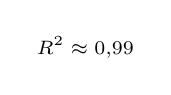
\begin{tikzpicture}[x=.5cm,y=.55cm,font=\scriptsize]
  \diagram{0}{1}{9}{0}{1}{6}
  \rechte{0}{9}{0.5}{1}
  \punten[inkt]{(1,1.6) (2,1.9) (3,2.6) (4,2.9) (5,3.4) (6,4.1) (7,4.4) (8,5.1)}
  \node[below] at (4.5,-.4) {$R^2 \approx 0{,}99$};
\end{tikzpicture}\qquad
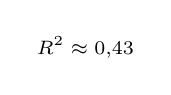
\begin{tikzpicture}[x=.5cm,y=.55cm,font=\scriptsize]
  \diagram{0}{1}{9}{0}{1}{6}
  \rechte{0}{9}{0.3917}{1.425}
  \punten[inkt]{(1,2.6) (2,0.9) (3,3.6) (4,1.6) (5,4.4) (6,3.1) (7,5.4) (8,3.9)}
  \node[below] at (4.5,-.4) {$R^2 \approx 0{,}43$};
\end{tikzpicture}}

Links verklaart de rechte bijna alles, rechts minder dan de helft: de punten liggen ver boven en onder de rechte, en de helling zelf is onzeker.

\voorbeeld{}{Bereken $R^2$ voor de tweedehandswagens uit hoofdstuk 1 (leeftijd en prijs), met $\Syy = 101{,}2$ en $\Qf \approx 0{,}367$. Wat betekent het getal?\label{vb:h2-r2}}{%
\uitleg{$\Qt$ is $\Syy$, en $\Qf$ is de kleinste kwadratensom. Met de tweede vorm van de formule is $\Qv$ niet nodig.}
\begin{stappenbreed}
R^2 = 1 - \frac{0{,}367}{101{,}2} \approx 0{,}996 & Het deel dat verklaard wordt.
\end{stappenbreed}
De leeftijd verklaart $99{,}6~\%$ van de variatie in de prijzen van deze vijf wagens. De rest, $0{,}4~\%$, komt van iets anders: de kilometerstand, opties, de staat van de wagen. Met \texttt{DiagnosticOn} toont \texttt{LinReg(ax+b)} hetzelfde getal als \texttt{r\textasciicircum 2}.}

\begin{oefeningen}
\oef{h2-r2}
\end{oefeningen}

\subsection{$R^2$ en de correlatiecoëfficiënt}

Het rekentoestel noemt het getal $r^2$, het kwadraat van de correlatiecoëfficiënt. Toeval?

\begin{theorie}
\begin{stelling}{Determinatie en correlatie}
\qquad $\formule{R^2 = r^2}$
\end{stelling}

\begin{bewijs}
Omdat $\yhat_i - \ybar = a x_i + b - (a\xbar + b) = a(x_i - \xbar)$, is
\bewijsregel{\Qv = a^2\som (x_i - \xbar)^2 = \frac{\Sxy^2}{\Sxx^2}\Sxx = \frac{\Sxy^2}{\Sxx} , \quad\text{dus}\quad R^2 = \frac{\Qv}{\Qt} = \frac{\Sxy^2}{\Sxx\Syy} = r^2 .}
\end{bewijs}
\end{theorie}

Twee gevolgen. Omdat $R^2 \leqslant 1$, is $r^2 \leqslant 1$: dat bewijst eindelijk dat $-1 \leqslant r \leqslant 1$, wat je in de 2de graad alleen zag. En $R^2$ zegt de sterkte, $r$ zegt ook de richting: $r = -0{,}9$ en $r = 0{,}9$ geven allebei $R^2 = 0{,}81$. Let op: $r = 0{,}7$ klinkt sterk, maar dan verklaart het model maar $49~\%$.

\voorbeeld{}{Bij een onderzoek naar de lengte van ouders en kinderen is $r = 0{,}5$. Welk deel van de variatie in de lengte van de kinderen verklaart de lengte van de ouders? Wat betekent dat?\label{vb:h2-r2r}}{%
\uitleg{We kwadrateren $r$, en vertalen het resultaat naar de context.}
\begin{stappenbreed}
R^2 = 0{,}5^2 = 0{,}25 & Het verklaarde deel.
\end{stappenbreed}
De lengte van de ouders verklaart een kwart van de variatie. De andere drie kwart komen van andere factoren, en van het toeval. \textit{Verklaren} betekent hier: statistisch voorspellen. Of het ook een oorzaak is (de genen), zegt $R^2$ niet.}

\begin{oefeningen}
\oef{h2-r2r}
\end{oefeningen}

%========================================================================================
\section{De residuen bekijken}

\subsection{De residuplot}

Een hoge $R^2$ betekent niet dat een rechte het juiste model is. Ook een kromme kan een hoge $R^2$ geven. Hoe zie je dat? Kijk naar wat de rechte \textit{niet} verklaart: de residuen. Past het model, dan zijn de residuen alleen toevallige fouten, zonder patroon.

\begin{theorie}
Een \textbf{\textcolor{accent}{residuplot}} is het spreidingsdiagram van de punten $\formule{(x_i, e_i)}$, met $e_i = y_i - \yhat_i$ het residu bij $x_i$.
\end{theorie}

Omdat $\som e_i = 0$ en $\som x_i e_i = 0$, ligt de residuplot altijd rond de horizontale as, zonder helling. De vraag is of er nog \textit{iets anders} in zit. De figuren tonen drie gevallen.

\figuren{\begin{tikzpicture}[x=.38cm,y=.5cm,font=\scriptsize]
  \draw[->,grijs] (0,0) -- (10,0) node[right,text=black] {$x$};
  \draw[->,grijs] (0,-2.2) -- (0,2.4) node[above,text=black] {$e$};
  \punten[inkt]{(1,0.6) (2,-0.9) (3,0.3) (4,1.2) (5,-0.4) (6,-1.1) (7,0.8) (8,-0.2) (9,0.5)}
  \node[below,align=center] at (5,-2.3) {geen patroon:\\de rechte past};
\end{tikzpicture}\qquad
\begin{tikzpicture}[x=.38cm,y=.5cm,font=\scriptsize]
  \draw[->,grijs] (0,0) -- (10,0) node[right,text=black] {$x$};
  \draw[->,grijs] (0,-2.2) -- (0,2.4) node[above,text=black] {$e$};
  \punten[inkt]{(1,1.6) (2,0.7) (3,-0.2) (4,-0.9) (5,-1.2) (6,-0.8) (7,-0.3) (8,0.6) (9,1.7)}
  \node[below,align=center] at (5,-2.3) {een boog:\\geen lineair verband};
\end{tikzpicture}\qquad
\begin{tikzpicture}[x=.38cm,y=.5cm,font=\scriptsize]
  \draw[->,grijs] (0,0) -- (10,0) node[right,text=black] {$x$};
  \draw[->,grijs] (0,-2.2) -- (0,2.4) node[above,text=black] {$e$};
  \punten[inkt]{(1,0.1) (2,-0.2) (3,0.4) (4,-0.6) (5,0.8) (6,-1.0) (7,1.4) (8,-1.7) (9,1.9)}
  \node[below,align=center] at (5,-2.3) {een trechter:\\spreiding groeit};
\end{tikzpicture}}

Een boog betekent dat de punten systematisch eerst boven, dan onder en dan weer boven de rechte liggen: het verband is gekromd, en een ander model past beter (hoofdstuk 3). Een trechter betekent dat de fouten groter worden met $x$: de rechte kan nog kloppen, maar een voorspelling is bij grote $x$ veel onzekerder. Een punt ver van de rest is een uitschieter, die je moet onderzoeken.

\voorbeeld{}{Bij een remproef meet men de remweg $y$ (in m) bij vijf snelheden $x$ (in m/s).

\smallskip
\kleinetabel[$x$ (m/s)][$y$ (m)]{5}{10 & 15 & 20 & 25 & 30}{6{,}2 & 13{,}1 & 24{,}5 & 37{,}0 & 54{,}3}

\smallskip
Bepaal de regressierechte en $R^2$. Teken de residuplot. Is een rechte een goed model?\label{vb:h2-residuplot}}{%
\naast{\uitleg{We laten ICT de rechte en de residuen berekenen (lijst \texttt{RESID}), en tekenen de punten $(x_i, e_i)$.}
\begin{stappenvrij}{5.5cm}{3cm}
\yhat = 2{,}402x - 21{,}02 & Met \texttt{LinReg(ax+b)}. \\[1ex]
R^2 \approx 0{,}976 & Hoog. \\[1ex]
e_i\colon\ 3{,}2;\ {-1{,}91};\ {-2{,}52};\ {-2{,}03};\ 3{,}26 & De residuen.
\end{stappenvrij}}{\begin{tabular}{@{}c@{}}\begin{tikzpicture}[x=.09cm,y=.035cm,font=\scriptsize]
  \diagram[$x$][$y$]{5}{5}{35}{-30}{10}{60}
  \xas{10,20,30}\yas{0,30,60}
  \rechte{5}{35}{2.402}{-21.02}
  \punten[inkt]{(10,6.2) (15,13.1) (20,24.5) (25,37.0) (30,54.3)}
\end{tikzpicture}\\[2mm]
\begin{tikzpicture}[x=.09cm,y=.38cm,font=\scriptsize]
  \draw[->,grijs] (5,0) -- (36,0) node[right,text=black] {$x$};
  \draw[->,grijs] (5,-3.5) -- (5,4) node[above,text=black] {$e$};
  \foreach \t in {-3,3}{\node[left] at (5,\t) {$\t$};}
  \punten[fel!80!black]{(10,3.2) (15,-1.91) (20,-2.52) (25,-2.03) (30,3.26)}
\end{tikzpicture}\end{tabular}}
Ondanks $R^2 \approx 0{,}976$ is de rechte geen goed model: de residuplot toont een duidelijke boog. Aan de randen ligt de remweg boven de rechte, in het midden eronder. De fysica zegt waarom: de remweg is evenredig met het kwadraat van de snelheid.}

\begin{werkwijze}
Teken altijd eerst het spreidingsdiagram, en na de regressie de residuplot. Zoek naar een boog (dan is het verband niet lineair), een trechter (de spreiding hangt af van $x$) en uitschieters. Zie je geen patroon, dan is een rechte een redelijk model, en zegt $R^2$ hoe goed ze de gegevens beschrijft.
\end{werkwijze}

\begin{oefeningen}
\oef{h2-residuplot}
\end{oefeningen}

\subsection{Het kwartet van Anscombe}

Hoe ver kan het gaan? De Britse statisticus Francis Anscombe publiceerde in 1973 vier kleine verzamelingen gegevens om te tonen dat getallen alleen niet volstaan. Ze hebben bijna precies hetzelfde gemiddelde punt $(9;\ 7{,}5)$, dezelfde regressierechte $\yhat = 0{,}5x + 3$, en dezelfde $R^2 \approx 0{,}67$. De figuren tonen de vier verzamelingen.

\figuren{\begin{tikzpicture}[x=.18cm,y=.22cm,font=\scriptsize]
  \diagram{2}{4}{20}{2}{4}{14}
  \xas{4,12,20}\yas{6,10,14}
  \rechte{3}{20}{0.5}{3}
  \punten[inkt]{(10,8.04) (8,6.95) (13,7.58) (9,8.81) (11,8.33) (14,9.96) (6,7.24) (4,4.26) (12,10.84) (7,4.82) (5,5.68)}
  \node[below] at (11,-0.2) {I};
\end{tikzpicture}\quad
\begin{tikzpicture}[x=.18cm,y=.22cm,font=\scriptsize]
  \diagram{2}{4}{20}{2}{4}{14}
  \xas{4,12,20}\yas{6,10,14}
  \rechte{3}{20}{0.5}{3}
  \punten[inkt]{(10,9.14) (8,8.14) (13,8.74) (9,8.77) (11,9.26) (14,8.10) (6,6.13) (4,3.10) (12,9.13) (7,7.26) (5,4.74)}
  \node[below] at (11,-0.2) {II};
\end{tikzpicture}\quad
\begin{tikzpicture}[x=.18cm,y=.22cm,font=\scriptsize]
  \diagram{2}{4}{20}{2}{4}{14}
  \xas{4,12,20}\yas{6,10,14}
  \rechte{3}{20}{0.5}{3}
  \punten[inkt]{(10,7.46) (8,6.77) (13,12.74) (9,7.11) (11,7.81) (14,8.84) (6,6.08) (4,5.39) (12,8.15) (7,6.42) (5,5.73)}
  \node[below] at (11,-0.2) {III};
\end{tikzpicture}\quad
\begin{tikzpicture}[x=.18cm,y=.22cm,font=\scriptsize]
  \diagram{2}{4}{20}{2}{4}{14}
  \xas{4,12,20}\yas{6,10,14}
  \rechte{3}{20}{0.5}{3}
  \punten[inkt]{(8,6.58) (8,5.76) (8,7.71) (8,8.84) (8,8.47) (8,7.04) (8,5.25) (19,12.50) (8,5.56) (8,7.91) (8,6.89)}
  \node[below] at (11,-0.2) {IV};
\end{tikzpicture}}

Alleen bij I is een rechte een redelijk model. Bij II liggen de punten op een kromme. Bij III liggen tien punten precies op een andere rechte, en trekt één uitschieter de regressierechte scheef. Bij IV bepaalt één punt alles: zonder het punt met $x = 19$ kun je geen rechte berekenen, want alle andere $x$ zijn gelijk. Zo'n punt, ver van de andere in de $x$-richting, heet een \textbf{invloedrijk punt}. Het besluit van Anscombe: teken altijd je gegevens. In opdracht \ref{oef:h2-o14} reken je het na.

%========================================================================================
\section{Is het verband echt?}

\subsection{Het regressiemodel}

Tot nu toe beschreven we gegevens. Maar meestal zijn de punten een \textit{steekproef}, en wil je iets zeggen over de hele populatie: over alle straten van de stad, alle tomatenplanten van de soort. Neem je een andere steekproef, dan krijg je een andere regressierechte. Hoe zeker is de helling dan? Daarvoor heb je een model nodig van hoe de gegevens ontstaan.

\begin{theorie}
Het \textbf{\textcolor{accent}{enkelvoudig lineair regressiemodel}} zegt dat bij elke $x_i$ de waarde $y_i$ toevallig is, met

\vspace{1mm}
\qquad $\formule{Y_i = \alpha x_i + \beta + \varepsilon_i}$

\vspace{1mm}
waarbij de \textbf{\textcolor{accent}{fouten}} $\varepsilon_1, \ldots, \varepsilon_n$ onafhankelijk zijn en normaal verdeeld met gemiddelde 0 en dezelfde standaardafwijking $\sigma$. De rechte $y = \alpha x + \beta$ is de \textbf{\textcolor{accent}{populatierechte}}.
\end{theorie}

Let op: in dit hoofdstuk is $\alpha$ de helling van de populatierechte, niet het significantieniveau van een toets. Dat noemen we daarom voluit.

\naast{\begin{minipage}{9.6cm}
De populatierechte ken je niet: de regressierechte $\yhat = ax + b$ schat haar uit de steekproef. Rechts zie je de populatierechte $y = 0{,}5x + 2$ (gestreept) en de regressierechten van zes steekproeven die een computer trok, elk met $x = 1, 2, \ldots, 8$ en $\sigma = 1$. Hun hellingen liggen tussen $0{,}41$ en $0{,}76$. De helling $a$ is zelf een toevalsvariabele, met een eigen spreiding. Hoe groot is die spreiding? Ze hangt af van de fouten (hoe groter $\sigma$, hoe onzekerder) en van de $x$-waarden (hoe verder ze uit elkaar liggen, hoe beter ze de helling vastleggen).
\end{minipage}}{\begin{tikzpicture}[x=.6cm,y=.42cm,font=\scriptsize]
  \diagram{0}{1}{9}{0}{2}{8}
  \xas{0,2,...,8}\yas{0,2,...,8}
  \foreach \a/\b in {0.586/1.628,0.465/2.416,0.762/0.241,0.405/2.698,0.541/1.782,0.456/1.873}{\rechte[accent!60]{0.5}{8.5}{\a}{\b}}
  \draw[inkt,very thick,dashed] (0.5,2.25) -- (8.5,6.25);
\end{tikzpicture}}

\subsection{De standaardfout van de helling}

De spreiding $\sigma$ van de fouten ken je niet: je schat ze met de residuen. Je deelt hun kwadratensom door $n - 2$, en niet door $n$. Zoals bij de steekproefstandaardafwijking (met $n - 1$) zijn de residuen kleiner dan de echte fouten, omdat de rechte zo goed mogelijk door de punten gaat. De residuen voldoen aan twee voorwaarden, $\som e_i = 0$ en $\som x_i e_i = 0$: er zijn maar $n - 2$ vrijheidsgraden.

\begin{theorie}
De \textbf{\textcolor{accent}{standaardfout van de residuen}} en de \textbf{\textcolor{accent}{standaardfout van de helling}} zijn

\vspace{1mm}
\qquad $\formule{s_e = \sqrt{\frac{\Qf}{n - 2}}}$ \quad en \quad $\formule{s_a = \frac{s_e}{\sqrt{\Sxx}}}$

\begin{stelling}{Verdeling van de helling}
In het regressiemodel heeft \quad $\formule{T = \frac{a - \alpha}{s_a}}$ \quad een t-verdeling met $\formule{n - 2}$ vrijheidsgraden.
\end{stelling}
\end{theorie}

De stelling bewijzen we niet: dat vraagt rekenregels voor sommen van toevalsvariabelen en de verdeling van $s_e$, die buiten het leerplan vallen. Ze lijkt wel op wat je kent uit Kansverdelingen: daar had $\frac{\xbar - \mu}{s/\sqrt n}$ een t-verdeling met $n - 1$ vrijheidsgraden. Ook de formule voor $s_a$ is te begrijpen: $s_e$ in de teller (meer ruis, meer onzekerheid), en $\sqrt{\Sxx}$ in de noemer (meer spreiding in $x$, minder onzekerheid).

\voorbeeld{}{Een tuinder geeft acht tomatenplanten elk een andere hoeveelheid water per dag $x$ (in liter), en weegt de oogst $y$ (in kg).

\smallskip
\kleinetabel[$x$ (l)][$y$ (kg)]{8}{0{,}5 & 0{,}8 & 1{,}0 & 1{,}2 & 1{,}5 & 1{,}8 & 2{,}0 & 2{,}4}{2{,}1 & 2{,}6 & 2{,}4 & 3{,}1 & 2{,}9 & 3{,}6 & 3{,}3 & 3{,}9}

\smallskip
Bereken de regressierechte, $s_e$ en $s_a$.\label{vb:h2-se}}{%
\uitleg{We berekenen $\Sxx$ en $\Sxy$ voor de rechte, de residuen voor $\Qf$, en dan de twee standaardfouten.}
\begin{stappenbreed}
\Sxx = 2{,}9, \quad \Sxy = 2{,}58, \quad a \approx 0{,}8897, \quad b \approx 1{,}742 & Met $\xbar = 1{,}4$ en $\ybar = 2{,}9875$. \\[1ex]
\Qf \approx 0{,}3134 & Som van de kwadraten van de residuen. \\[1ex]
s_e = \sqrt{\tfrac{0{,}3134}{6}} \approx 0{,}2286 & Met $n - 2 = 6$. \\[1ex]
s_a = \tfrac{0{,}2286}{\sqrt{2{,}9}} \approx 0{,}134 & De standaardfout van de helling.
\end{stappenbreed}
De oogst stijgt volgens de steekproef met $0{,}89$~kg per liter, met een standaardfout van $0{,}13$~kg per liter. \texttt{LinRegTTest} geeft $s_e$ als \texttt{s}.}

\begin{oefeningen}
\oef{h2-se}
\end{oefeningen}

\subsection{Een toets voor de helling}

Is er wel een verband? Als $\alpha = 0$, hangt $Y$ in het model niet van $x$ af. De helling $a$ van de steekproef is dan alleen door toeval verschillend van 0. Dat toets je zoals in Kansverdelingen.

\begin{theorie}
De \textbf{\textcolor{accent}{t-toets voor de helling}} toetst $H_0\colon \alpha = 0$ (geen lineair verband) met de toetsingsgrootheid

\vspace{1mm}
\qquad $\formule{t = \frac{a}{s_a}}$

\vspace{1mm}
Als $H_0$ waar is, komt $t$ uit $\formule{t_{n-2}}$. De p-waarde is de oppervlakte onder $t_{n-2}$ voorbij $t$, in de richting van $H_1$; bij $H_1\colon \alpha \neq 0$ verdubbel je ze.
\end{theorie}

\voorbeeld{}{Is er bij de tomatenplanten een verband tussen water en oogst? Toets met significantieniveau $0{,}05$.\label{vb:h2-toets}}{%
\uitleg{We toetsen tweezijdig of de populatiehelling 0 is, met $n - 2 = 6$ vrijheidsgraden.}
\naast{\begin{stappenvrij}{5.6cm}{3.6cm}
H_0\colon \alpha = 0 \qquad H_1\colon \alpha \neq 0 & Tweezijdig. \\[1ex]
t = \frac{0{,}8897}{0{,}1342} \approx 6{,}63 & Met $s_a$ uit voorbeeld \ref{vb:h2-se}. \\[1.5ex]
\text{p-waarde} = 2P(T \geqslant 6{,}63) \approx 0{,}0006 & \texttt{2*tcdf(6.63,1E99,6)}. \\[1ex]
0{,}0006 \leqslant 0{,}05\colon\ H_0 \text{ verwerpen} & Significant.
\end{stappenvrij}}{\begin{tikzpicture}[x=.24cm,y=7cm,font=\scriptsize]
  \draw[accent,thick] plot[domain=-7.5:7.5,samples=80,smooth] (\x,{tdich(\x,6)});
  \kansassen{-7.5}{7.9}{.44}{$t$}
  \draw[fel!80!black,thick] (6.63,0) -- (6.63,.12) node[above,text=black] {$6{,}63$};
  \draw[fel!80!black,thick] (-6.63,0) -- (-6.63,.12) node[above,text=black] {$-6{,}63$};
  \node[below] at (0,0) {0};
\end{tikzpicture}}
De waarde 6,63 ligt zo ver in de staart dat de oppervlakte voorbij $\pm 6{,}63$ niet te zien is. Er is dus wel degelijk een verband: meer water gaat samen met een grotere oogst. \texttt{LinRegTTest} (met $\beta$ \& $\rho \neq 0$) geeft meteen $t \approx 6{,}63$ en $p \approx 0{,}0006$.}

Een kleine p-waarde zegt dat de helling niet 0 is, niet dat ze groot is, en ook niet dat $x$ de oorzaak is. Hier gaf de tuinder zelf het water: dat is een experiment, en dan mag je wel over een oorzaak spreken, als de planten aselect over de hoeveelheden verdeeld zijn.

\begin{werkwijze}
\textbf{1.}~Teken het spreidingsdiagram en de residuplot, en controleer de voorwaarden (onafhankelijke waarnemingen, een lineair verband, geen trechter, geen sterke uitschieters). \ \textbf{2.}~Formuleer $H_0\colon \alpha = 0$ en $H_1$ ($\alpha \neq 0$, of eenzijdig $\alpha > 0$ of $\alpha < 0$). \ \textbf{3.}~Bereken $a$, $s_a$ en $t = \frac{a}{s_a}$ met $n - 2$ vrijheidsgraden, of laat \texttt{LinRegTTest} alles doen. \ \textbf{4.}~Vergelijk de p-waarde met het significantieniveau, en besluit in de context.
\end{werkwijze}

\begin{oefeningen}
\oef{h2-toets}
\end{oefeningen}

\needspace{14\baselineskip}
\subsection{Een betrouwbaarheidsinterval voor de helling}

Een toets zegt alleen of de helling 0 kan zijn. Wil je weten hoe groot ze ongeveer is, dan maak je een interval, zoals voor een gemiddelde.

\begin{theorie}
Een \textbf{\textcolor{accent}{95~\%-betrouwbaarheidsinterval}} voor de helling $\alpha$ van de populatierechte is

\vspace{1mm}
\qquad $\formule{\bigl[a - t^* s_a,\ a + t^* s_a\bigr]}$ \quad met \quad $\formule{t^* = \texttt{invT(0.975},n - 2\texttt{)}}$
\end{theorie}

Het interval volgt uit de stelling over de verdeling van de helling, net zoals in Kansverdelingen: $-t^* \leqslant \frac{a - \alpha}{s_a} \leqslant t^*$ betekent precies dat $\alpha$ in het interval ligt. Ligt 0 niet in het interval, dan verwerpt de tweezijdige toets $H_0\colon \alpha = 0$ bij significantieniveau $0{,}05$.

\voorbeeld{}{Bereken een 95~\%-betrouwbaarheidsinterval voor de helling bij de tomatenplanten.\label{vb:h2-interval}}{%
\uitleg{Met 6 vrijheidsgraden is $t^*$ groter dan 1,96. Heb je alleen de uitvoer van \texttt{LinRegTTest}, dan vind je $s_a$ als $\frac{a}{t}$.}
\begin{stappenbreed}
t^* = \texttt{invT(0.975,6)} \approx 2{,}447 & De kritieke waarde. \\[1ex]
0{,}8897 \pm 2{,}447 \cdot 0{,}1342 = 0{,}8897 \pm 0{,}328 & De foutenmarge. \\[1ex]
[0{,}56;\ 1{,}22] & In kg per liter.
\end{stappenbreed}
Met 95~\% betrouwbaarheid levert een liter water per dag extra tussen 0,56 en 1,22~kg tomaten meer op, binnen het onderzochte gebied van 0,5 tot 2,4 liter. Het interval bevat 0 niet, zoals de toets al zei.}

\begin{oefeningen}
\oef{h2-interval}

\oef{h2-voorwaarden}
\end{oefeningen}

%========================================================================================
\needspace{16\baselineskip}
\subsection{Terug naar het probleem}

Nu kunnen we de drie vragen over het bladerdek beantwoorden.

\voorbeeld{}{Terug naar het probleem. Welk deel van de variatie in temperatuur verklaart het bladerdek? Is het verband significant bij een significantieniveau van $0{,}05$? Hoeveel graden koeler is een straat met 10 procentpunt meer bladerdek, met 95~\% betrouwbaarheid?\label{vb:h2-terug}}{%
\uitleg{We laten ICT de rechte en de residuen berekenen, kijken naar de residuplot, en berekenen dan $R^2$, de toets en het interval.}
\naast{\begin{stappenvrij}{5.6cm}{3.4cm}
\yhat \approx -0{,}04817x + 35{,}34 & \texttt{LinReg(ax+b)}. \\[1ex]
R^2 \approx 0{,}858 & $r \approx -0{,}926$. \\[1ex]
s_e = \sqrt{\tfrac{\Qf}{8}} \approx 0{,}4435 & Met $\Qf \approx 1{,}574$. \\[1ex]
s_a = \tfrac{0{,}4435}{\sqrt{4088{,}5}} \approx 0{,}00694 & Met $\Sxx = 4088{,}5$. \\[1ex]
t = \tfrac{-0{,}04817}{0{,}00694} \approx -6{,}95 & Met $n - 2 = 8$. \\[1ex]
\text{p-waarde} \approx 0{,}0001 & Tweezijdig. \\[1ex]
t^* \approx 2{,}306\colon\ [-0{,}064;\ -0{,}032] & Interval voor $\alpha$.
\end{stappenvrij}}{\begin{tabular}{@{}c@{}}\begin{tikzpicture}[x=.05cm,y=.55cm,font=\scriptsize]
  \diagram[$x$][$y$]{0}{10}{70}{31}{1}{36}
  \xas{0,30,60}\yas{31,33,35}
  \rechte{0}{72}{-0.04817}{35.3401}
  \punten[inkt]{(5,35.3) (12,34.5) (18,34.9) (25,33.5) (30,34.0) (38,33.9) (45,32.9) (52,32.4) (60,33.1) (70,31.8)}
\end{tikzpicture}\\[2mm]
\begin{tikzpicture}[x=.05cm,y=1.1cm,font=\scriptsize]
  \draw[->,grijs] (0,0) -- (74,0) node[right,text=black] {$x$};
  \draw[->,grijs] (0,-.8) -- (0,.9) node[above,text=black] {$e$};
  \foreach \t/\l in {-.5/{-0,5},.5/{0,5}}{\node[left] at (0,\t) {$\l$};}
  \punten[fel!80!black]{(5,0.201) (12,-0.262) (18,0.427) (25,-0.636) (30,0.105) (38,0.39) (45,-0.272) (52,-0.435) (60,0.65) (70,-0.168)}
\end{tikzpicture}\end{tabular}}
De residuplot toont geen boog en geen trechter: een rechte is een redelijk model. Het bladerdek verklaart ongeveer 86~\% van de verschillen in temperatuur tussen de tien straten. Met een p-waarde van ongeveer $0{,}0001$ is het verband zeker geen toeval. Per 10 procentpunt meer bladerdek is de straat volgens de steekproef $0{,}48$~°C koeler, en met 95~\% betrouwbaarheid tussen $0{,}32$ en $0{,}64$~°C. Maar dit is observationeel onderzoek: straten met veel bomen zijn misschien ook breder of liggen dichter bij een park. Dat de bomen de oorzaak zijn, is aannemelijk, maar volgt niet uit deze gegevens.}

%========================================================================================
\opdrachtenkop

\begin{oefeningen}
\oef{h2-o1}

\needspace{10\baselineskip}
\oef{h2-o2}

\oef{h2-o3}

\needspace{10\baselineskip}
\oef{h2-o4}

\oef{h2-o5}

\needspace{12\baselineskip}
\oef{h2-o6}

\oef{h2-o7}

\needspace{12\baselineskip}
\oef{h2-o8}

\oef{h2-o9}

\needspace{12\baselineskip}
\oef{h2-o10}

\oef{h2-o11}

\needspace{12\baselineskip}
\oef{h2-o12}

\oef{h2-o13}

\needspace{16\baselineskip}
\oef{h2-o14}

\oef{h2-o15}

\needspace{12\baselineskip}
\oef{h2-o16}

\oef{h2-o17}

\needspace{12\baselineskip}
\oef{h2-o18}

\oef{h2-o19}

\needspace{12\baselineskip}
\oef{h2-o20}

\oef{h2-o21}

\needspace{12\baselineskip}
\oef{h2-o22}
\end{oefeningen}

%----------------------------------------------------------------------------------------
% KOPPEL: verbanden met andere leerstof
%----------------------------------------------------------------------------------------
\needspace{20\baselineskip}
\opdrachtsectie{Koppel}

\lkr{De eerste oefening steunt op het scalair product en de stelling van Pythagoras in de ruimte (Ruimtemeetkunde, hoofdstuk 4), de tweede op Statistiek (hoofdstuk 1: samenhang en causaliteit) en de derde op Kansverdelingen (hoofdstuk 3, de t-toets voor een gemiddelde).}

\begin{oefeningen}
\oef{h2-koppel-1}

\oef{h2-koppel-2}

\oef{h2-koppel-3}
\end{oefeningen}

%----------------------------------------------------------------------------------------
\opdrachtsectie{Test jezelf}

\begin{oefeningen}
\oef{h2-t1}

\oef{h2-t2}

\oef{h2-t3}

\oef{h2-t4}

\oef{h2-t5}

\oef{h2-t6}

\oef{h2-t7}
\end{oefeningen}

\herhaalschema{%
  \fv{oef:h2-t1}{vb:h2-drie}{oef:h2-drie}%
  \fv{oef:h2-t2}{vb:h2-r2}{oef:h2-r2}%
  \fv{oef:h2-t3}{vb:h2-r2r}{oef:h2-r2r}%
  \fv{oef:h2-t4}{vb:h2-residuplot}{oef:h2-residuplot}%
  \fv{oef:h2-t5}{vb:h2-se}{oef:h2-se}%
  \fv{oef:h2-t6}{vb:h2-toets}{oef:h2-toets}%
  \fv{oef:h2-t7}{vb:h2-interval}{oef:h2-interval}}

\ifzelfstudie
\section*{Maak je eigen samenvatting}
Sluit dit boek en schrijf in je schrift: de drie kwadratensommen met hun betekenis en een figuur, de splitsing $\Qt = \Qv + \Qf$ met het bewijs, de definitie van $R^2$ en wat het getal betekent, waarom $R^2 = r^2$ en waarom daaruit $-1 \leqslant r \leqslant 1$ volgt, wat een residuplot is en welke patronen je zoekt, wat het kwartet van Anscombe leert, het regressiemodel met zijn voorwaarden, $s_e$ en $s_a$ (en waarom $n - 2$), de t-toets voor de helling en het betrouwbaarheidsinterval voor de helling, en waarom een significant verband nog geen oorzaak is. Vergelijk daarna met de kaders.
\fi
